\chapter{Result and Discussion}
\label{Chapter7}

\large {



\section{Abstract}
Paper abstract goes here
\section{Paper Section}
Section stuff

\subsection{Paper Subsection}
\section{Paper Section}
Section stuff

\subsection{Paper Subsection}
\section{Paper Section}
Section stuff

\subsection{Paper Subsection}

\subsection{Paper Subsection}
\section{Final Paper Section}
Wrap up your paper here

\section{Acknowledgments}
Put the acknowledgements from your paper here



 and measuring the HI emissions' closure phase.


The feed horn testing results demonstrate that the power level received and analysed by the SA was the same as that generated by the SG, as shown in figure, indicating that the feed horn design was successful.

Antenna control system power cables and the front-end electronics cables were successfully laid.
Construction of a power supply system and building of a rack unit for the antenna controllers, receiver unit, and front and back-end electronics has been completed.
The design and construction of the mini power distribution station were successfully completed.
The radio frequency (RF) cables from the lab to each of the antennas were phased out and laid.
The prototyping of the feed horn design, fabricating, and testing was successfully completed.
 
 







\section{Result}

\subsection{Construction of New RC Structure and Reinforcement}
Figure 7  shows the construction of the RC Reinforcement for the concrete platform.

\begin{figure}[htp]
\includegraphics[width=3in]{New_RC_Structure_Reinforcement.jpg}
\includegraphics[width=3in]{New_C_Structure _Reinforcement.jpg}
\caption{Construction of the RC Structure Reinforcement}
\label{fig:galaxy}
%\end{figure}

 \vspace{0.5cm}
 
%\begin{figure}[htp]
   % \centering
    \textbf{Figure 8 shows the construction of the Concrete Platform for the Antenna column}
    
 \includegraphics[width=3in]{Concrete_plateform1.jpg}  
\includegraphics[width=3in]{Concrete_Platform4.jpg}
\caption{Construction of Antenna Base Concrete
Platform}
\label{fig:galaxy}
\end{figure}

\vspace{1cm}

\subsection{Dish Bracket 3D Design and Fabrication}

Figure shown 3D design of the 2.4m dish Brackets and the metal galvanise Fabrications.

\begin{figure}[htp]
    \centering
\includegraphics[width=2.5in]{3D Bracket_front_half_view.png}
 \includegraphics[width=2.5in]{3D Bracket_front_view.png}
    \includegraphics[width=2.5in]{3D Bracket_side_view2.png}
    \includegraphics[width=2.5in]{3D Bracket_real_view.png}
    \caption{3D Design of the Dish Bracket}
    \label{fig:galaxy}
%\end{figure}
\vspace{0.5cm}
%\begin0.5cm{figure}[htp]
    \centering
    \includegraphics[width=3in]{Dish_BRACKET2.jpg}
    \includegraphics[width=3in]{Dish_bracket.jpg}
    \caption{Fabrication of the Dish Bracket}
    \label{fig:galaxy}
\end{figure}

\vspace{1cm}

\subsection{Fabrication of the Antenna Columns}
Figure 14 shows the 3D Design and the Fabricated Antenna column.
\begin{figure}[htp]
    \centering
\includegraphics[width=3in]{3D_TOWER.png}
\caption{3D Design of the Antenna Column or Tower}
\label{fig:galaxy }

\includegraphics[width=2in]{conlumn_fabrication2.jpg} 
\includegraphics[width=3in]{column_fabrication1.jpg}
\caption{Antenna Column Fabrication}
\label{fig:galaxy }
\end{figure}

\vspace{1cm}

\subsection{Telescope Prototype Assembling }

 Figure 16 to 18 below show the full 3D Design of the 2.4m dish antenna showing the control system and the counter weight.

\begin{figure}[htp]
    \centering
 \includegraphics[width=2.5in]{3D Design_counter_weight_view.png}
  \includegraphics[width=2.5in]{3D Design_bracket_view.png}
   \includegraphics[width=2.5in]{3D Design_dish_view.png}
 \includegraphics[width=2.5in]{3D Design_feed_view.png}
 \caption{3D Designs of the Telescope }
    \label{fig:galaxy}
\end{figure}

\begin{figure}[htp]
    \centering
    \textbf{Figure 14 shows the first Telescope prototype-Testing with the control system.}
    
    \vspace{1cm}
    
 \includegraphics[width=3in]{telesscope_construction.jpg}
\includegraphics[width=3in]{Telescope_prototype_testing.jpg}
\caption{First Telescope Prototype Assembling}
  \label{fig:galaxy}
%\end{figure}
\vspace{1cm}

%\begin{figure}[htp]
    %\centering
\textbf{Figure 15m shows the assembling of the second Telescope prototype with the designed antenna column and the control system.} 
\vspace{0.5cm} 
    
\includegraphics[width=2.5in]{Telescope_Prototype5.jpg}
\includegraphics[width=2.5in]{Telescope_Prototype8.jpg}
\caption{Second Telescope Prototype Assembling}
    \label{fig:galaxy}
\end{figure}


\subsection{Conference Presentation}
Part of the 12 months period was also spent preparing for SAAO 200 Virtual Symposium which was presented via video conference. The title of the presentation was ’Developing an Array of Small Parabolic Antenna at MRT Site for Radio Astronomy Experiment (DASPA)’ and was presented at the ’SAAO 200 Virtual Symposium Organiser African Agenda’ in October 2020 \cite{Forson2020SAAO200}.





\section{Civil Designs 
and Engineering}
Section stuff

\subsection{Paper Subsection}
\section{Paper Section}
Section stuff

\subsection{Paper Subsection}

\subsection{Paper Subsection}
\section{Final Paper Section}
Wrap up your paper here

\section*{Acknowledgements}
Put the acknowledgements from your paper here





\section{Dish Bracket Design}
The dish bracket is the part that holds the symmetric reflectors together as a unit and firmly attached to the rotor and connected to the antenna column. The bracket also prevents the reflector from wind load damage or surface deformation.


\subsection{Designing of Dish Bracket}
The existing offset parabolic dishes requires new brackets that will conformed to the new design.
Three methods were experimented to be able to obtained error-free dish brackets design. The three experimented methods as follows below:
\begin{enumerate}[label=\alph*.]
\item Method 1:
Detail Sketch drawings of each symmetrical parts of the dish  
\item Method 2:
3D design drawings of the bracket  with SolidWorks simulation software.
\item Method 3:
Fabrication experimentation of step 1 and step 2
\end{enumerate}
The results section shows the three methods deployed under the section.









\subsection{Designing of the Existing and New RC Structure}

\begin{figure}[htp]
\vspace*{-1cm}
\makebox[\linewidth]{\includegraphics[width=1.3\linewidth]{PROPOSED ANTENNA BASE FOR MRT AT BRAS D'EAU-Model1.pdf}}
\caption{3D VIEW OF THE EXISTING AND RC STRUCTURE}
\end{figure}
 
 \newpage
 
\subsubsection{Designing of the Antenna Base Platform}
\begin{figure}[htp]
\vspace*{-1cm}
\makebox[\linewidth]{ \includegraphics[width=1.3\linewidth]{PROPOSED ANTENNA BASE FOR MRT AT BRAS D'EAU-Model2.pdf}}
    \caption{Antenna Base Platform View}
\end{figure}

\newpage
\subsubsection{Designing of the Antenna Base Plate Connection into the RC Structure}
\begin{figure}[htp]
\vspace*{-1cm}
\makebox[\linewidth]{ \includegraphics[width=1.3\linewidth]{PROPOSED ANTENNA BASE FOR MRT AT BRAS D'EAU-Model3.pdf}}
    \caption{New RC Structure Reinforcement}
\end{figure}


\subsubsection{Designing of the New RC Structure Reinforcement}

\begin{figure}[htp]
\vspace*{-1cm}
\makebox[\linewidth]{ \includegraphics[width=1.3\linewidth]{PROPOSED ANTENNA BASE FOR MRT AT BRAS D'EAU-Model4.pdf}}
    \caption{Tower Column RC Structure Connection To Base Plate 3D View}
\end{figure}


















 \begin{figure}[htp]
    \centering
    %\hfill
    \subfloat[Finding the feed focal point with ropes]
    {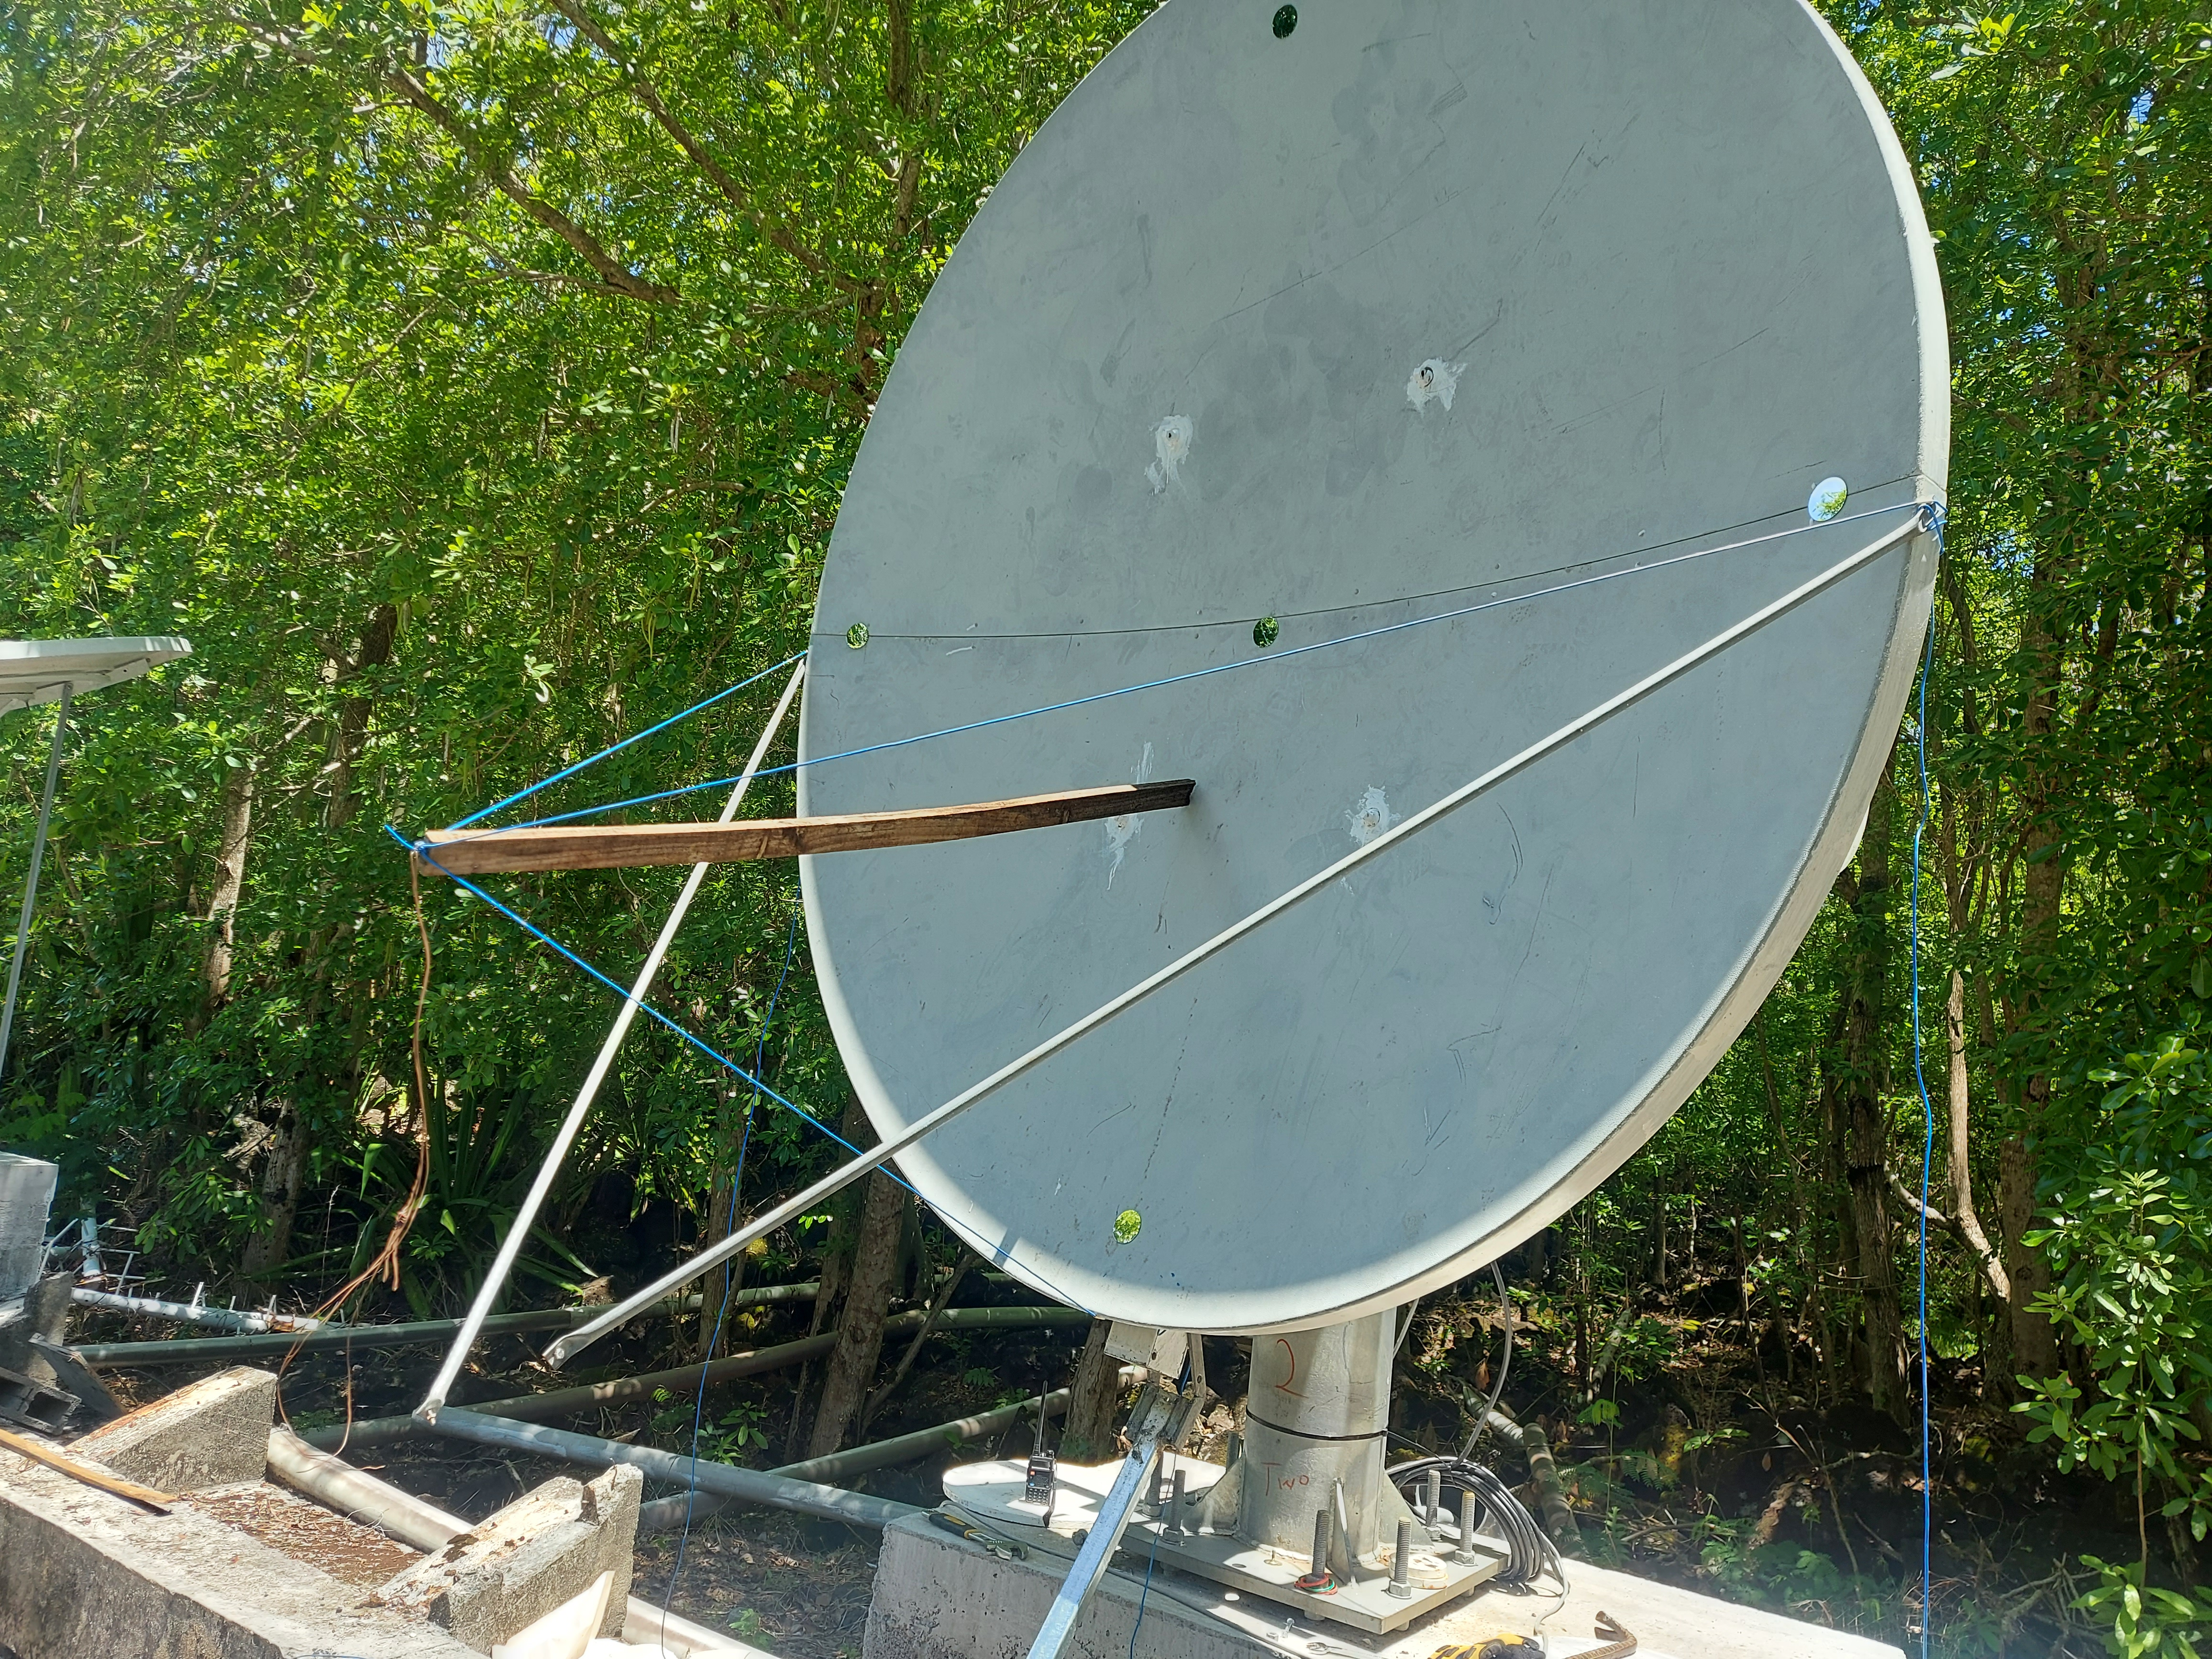
\includegraphics[width=2.5in]{Figures/Feed_focal_point.jpg}}
    \subfloat[Installation of the feed horn]
    {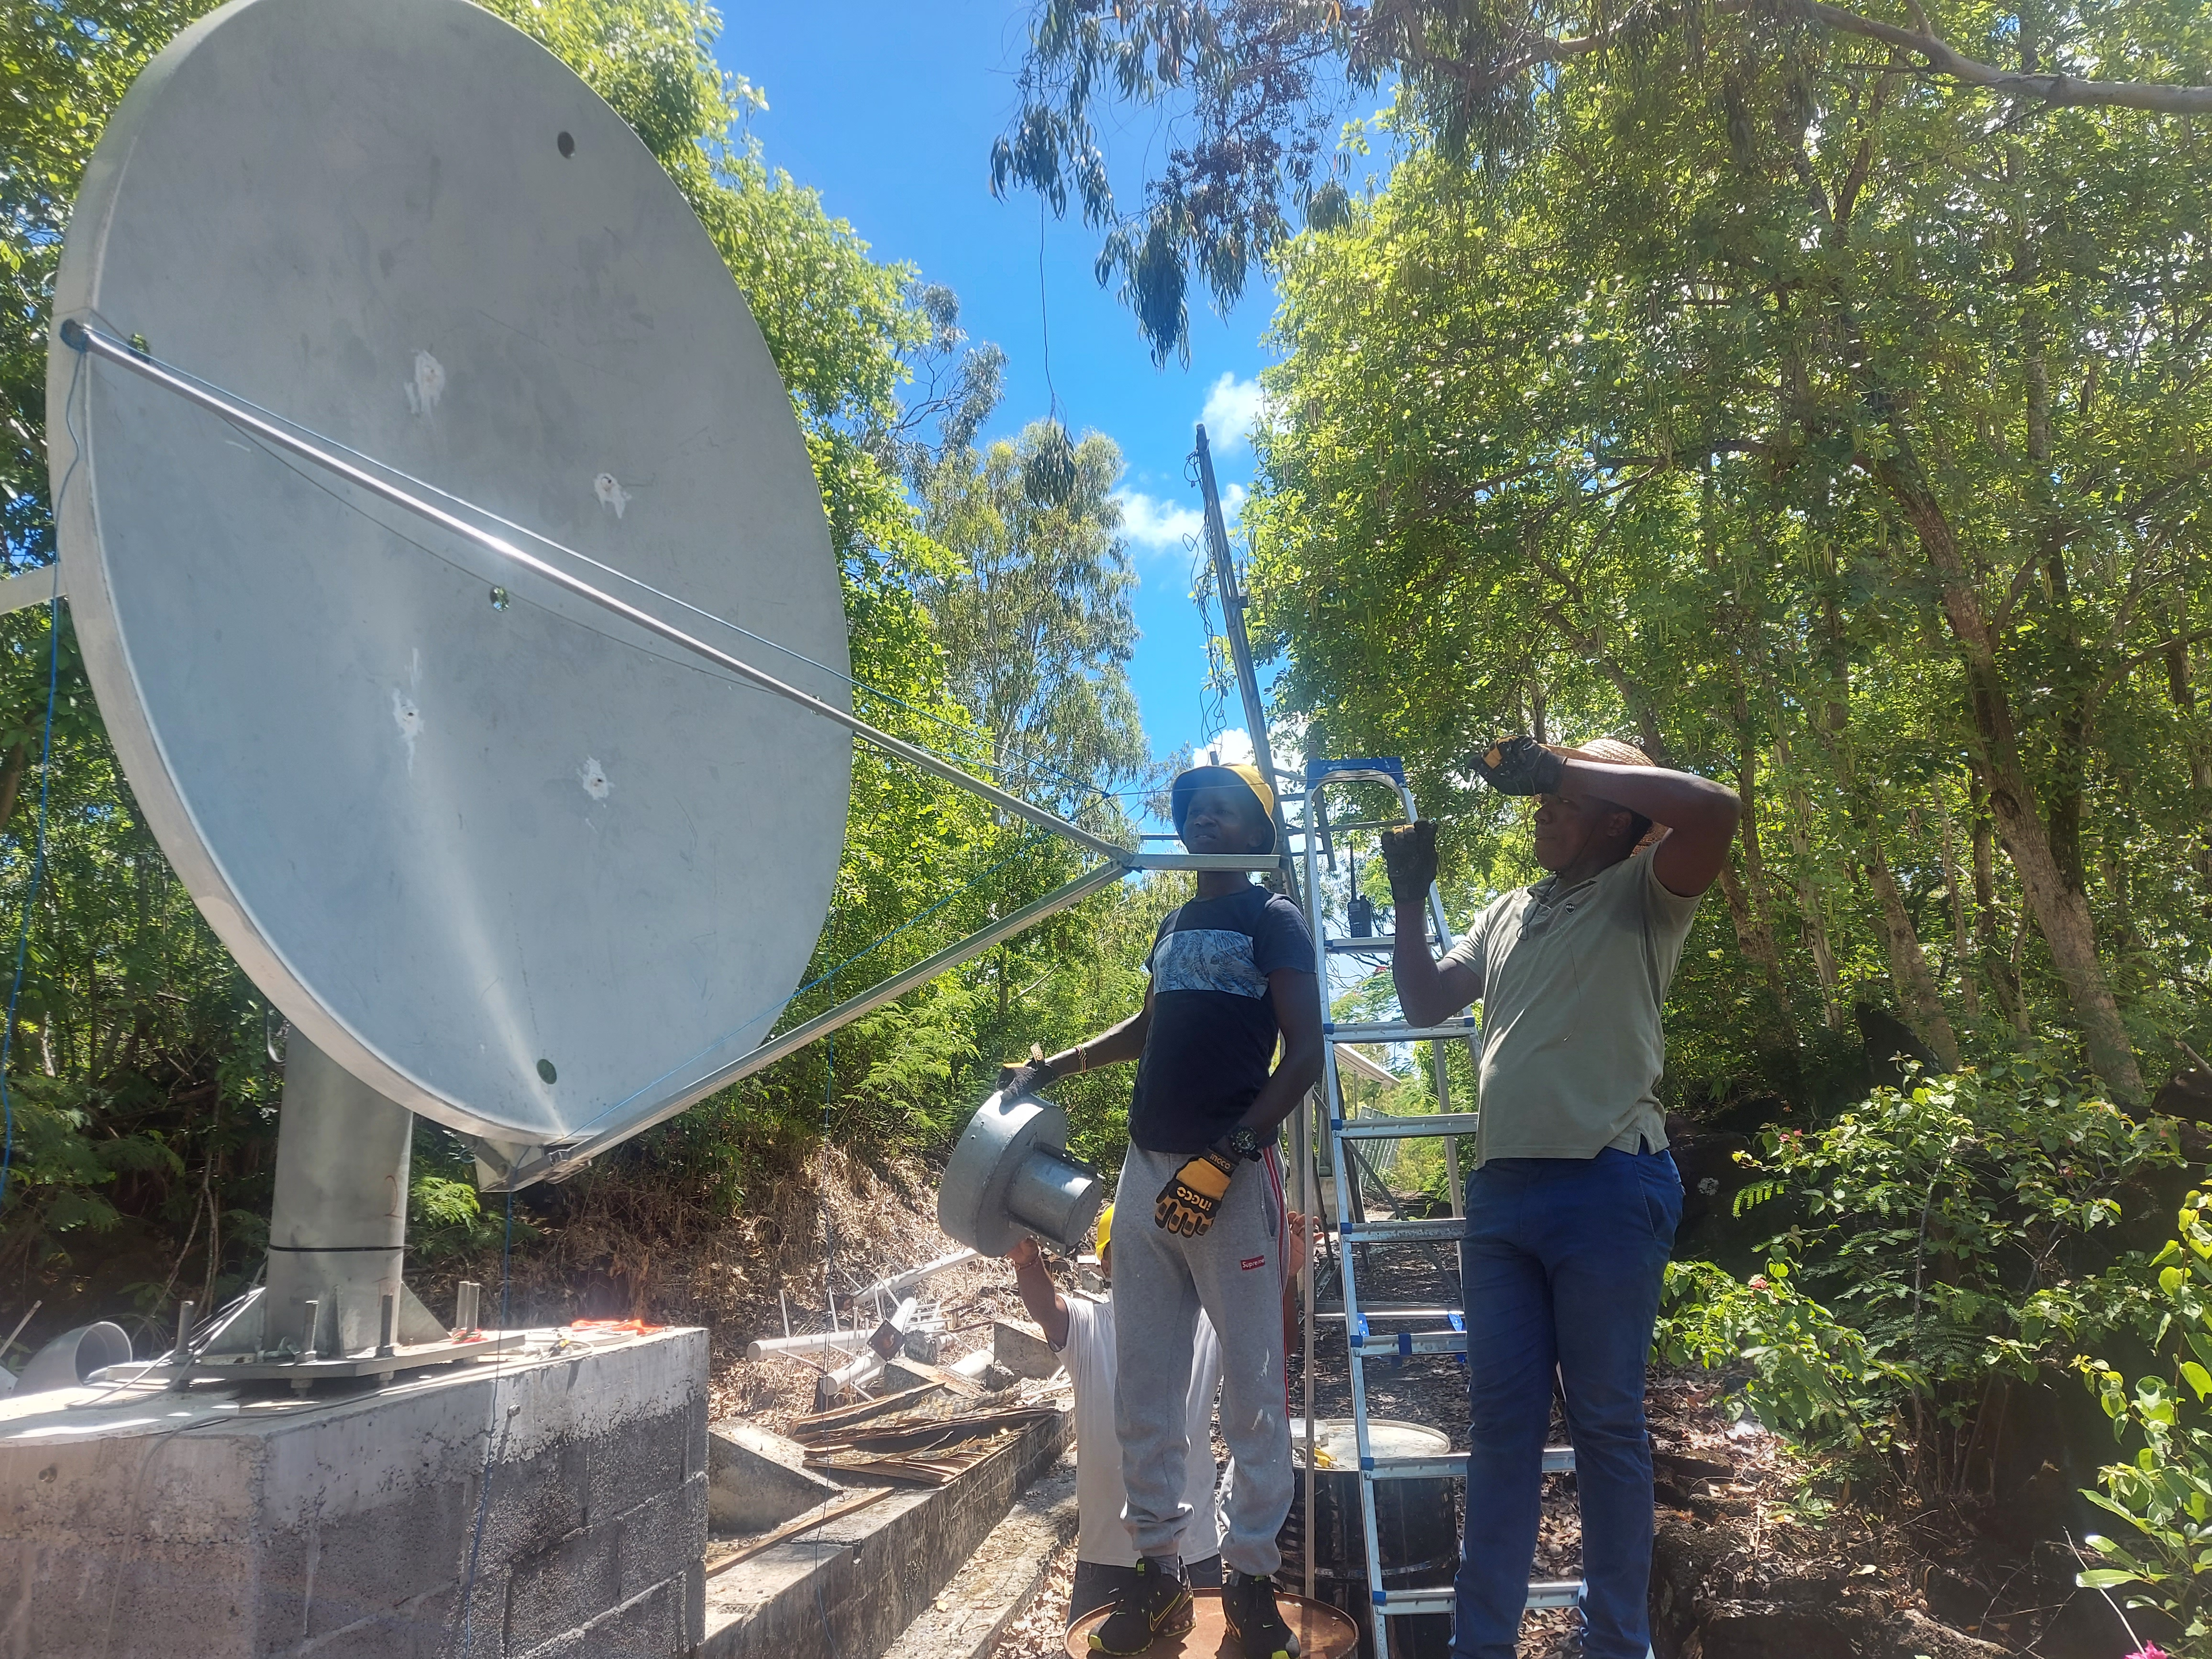
\includegraphics[width=2.5in]{Figures/Feed_suport_installation.jpg}}
    \caption{Installation of the feed horn and Feed supports arms}
    \label{fig:3.4}
\end{figure}
}